% ============================================================
% Lecture deck — Module 16 / Notebook 50
% Architecture Patterns for AI Applications
% HSBI house style. English content. TikZ visuals.
% The notebook is the single source of truth.
% ============================================================
\documentclass[aspectratio=169,11pt]{beamer}

\usepackage[utf8]{inputenc}
\usepackage[T1]{fontenc}
\usepackage{lmodern}
\usepackage[english]{babel}
\usepackage{graphicx}
\usepackage{booktabs}
\usepackage{amsmath,amssymb}
\usepackage{xcolor}
\usepackage{tikz}
\usetikzlibrary{positioning,arrows.meta,shapes.geometric,calc,fit,backgrounds}

% Speaker notes. Default build = clean slides, unchanged. For presenter view
% (slide left, notes right) build with:
%   pdflatex "\def\notesmode{}% ============================================================
% Lecture deck — Module 16 / Notebook 50
% Architecture Patterns for AI Applications
% HSBI house style. English content. TikZ visuals.
% The notebook is the single source of truth.
% ============================================================
\documentclass[aspectratio=169,11pt]{beamer}

\usepackage[utf8]{inputenc}
\usepackage[T1]{fontenc}
\usepackage{lmodern}
\usepackage[english]{babel}
\usepackage{graphicx}
\usepackage{booktabs}
\usepackage{amsmath,amssymb}
\usepackage{xcolor}
\usepackage{tikz}
\usetikzlibrary{positioning,arrows.meta,shapes.geometric,calc,fit,backgrounds}

% Speaker notes. Default build = clean slides, unchanged. For presenter view
% (slide left, notes right) build with:
%   pdflatex "\def\notesmode{}% ============================================================
% Lecture deck — Module 16 / Notebook 50
% Architecture Patterns for AI Applications
% HSBI house style. English content. TikZ visuals.
% The notebook is the single source of truth.
% ============================================================
\documentclass[aspectratio=169,11pt]{beamer}

\usepackage[utf8]{inputenc}
\usepackage[T1]{fontenc}
\usepackage{lmodern}
\usepackage[english]{babel}
\usepackage{graphicx}
\usepackage{booktabs}
\usepackage{amsmath,amssymb}
\usepackage{xcolor}
\usepackage{tikz}
\usetikzlibrary{positioning,arrows.meta,shapes.geometric,calc,fit,backgrounds}

% Speaker notes. Default build = clean slides, unchanged. For presenter view
% (slide left, notes right) build with:
%   pdflatex "\def\notesmode{}% ============================================================
% Lecture deck — Module 16 / Notebook 50
% Architecture Patterns for AI Applications
% HSBI house style. English content. TikZ visuals.
% The notebook is the single source of truth.
% ============================================================
\documentclass[aspectratio=169,11pt]{beamer}

\usepackage[utf8]{inputenc}
\usepackage[T1]{fontenc}
\usepackage{lmodern}
\usepackage[english]{babel}
\usepackage{graphicx}
\usepackage{booktabs}
\usepackage{amsmath,amssymb}
\usepackage{xcolor}
\usepackage{tikz}
\usetikzlibrary{positioning,arrows.meta,shapes.geometric,calc,fit,backgrounds}

% Speaker notes. Default build = clean slides, unchanged. For presenter view
% (slide left, notes right) build with:
%   pdflatex "\def\notesmode{}\input{50_architecture_patterns.tex}"
\ifdefined\notesmode
  \usepackage{pgfpages}
  \setbeameroption{show notes on second screen=right}
\fi

\usetheme{Madrid}
\usecolortheme{default}
\setbeamertemplate{navigation symbols}{}
\setbeamertemplate{footline}[frame number]
\setbeamertemplate{blocks}[rounded][shadow=false]
\setbeamertemplate{headline}{%
  \leavevmode%
  \hbox{%
    \begin{beamercolorbox}[wd=\paperwidth,ht=2.5ex,dp=1.125ex]{section in head/foot}%
      \insertsectionnavigationhorizontal{\paperwidth}{}{\hskip0pt plus1filll}%
    \end{beamercolorbox}%
  }%
}
\AtBeginSection[]{%
  \begin{frame}{Outline}
    \tableofcontents[currentsection,sectionstyle=show/shaded,subsectionstyle=show/show/hide]
  \end{frame}
}

\definecolor{hsbiblue}{RGB}{45,57,120}
\definecolor{hsbimid}{RGB}{76,114,176}
\definecolor{hsbilight}{RGB}{225,231,247}
\definecolor{cgreen}{RGB}{85,164,103}
\definecolor{corange}{RGB}{221,132,82}
\definecolor{cred}{RGB}{196,78,82}
\definecolor{cpurple}{RGB}{129,114,178}
\tikzset{
  box/.style={rounded corners=3pt, draw=hsbiblue, line width=1pt, fill=hsbilight, align=center, inner sep=5pt, font=\footnotesize},
  tier/.style={rounded corners=3pt, draw=hsbiblue, line width=1.2pt, fill=hsbilight, align=center, text width=2.5cm, minimum height=1.2cm, font=\footnotesize},
  flow/.style={rounded corners=2pt, draw=hsbiblue, line width=0.9pt, fill=hsbilight, align=center, text width=1.55cm, minimum height=0.85cm, font=\scriptsize},
  arr/.style={-{Stealth[length=2.6mm]}, line width=1pt, draw=hsbiblue},
}

% ---- Python code listings ----------------------------------
\usepackage{listings}
\lstdefinestyle{py}{%
  language=Python,
  basicstyle=\ttfamily\footnotesize,
  keywordstyle=\color{hsbiblue}\bfseries,
  commentstyle=\color{gray}\itshape,
  stringstyle=\color{cgreen!60!black},
  showstringspaces=false,
  columns=fullflexible,
  breaklines=true,
  aboveskip=3pt, belowskip=1pt,
}

\title{Architecture Patterns for AI Applications}
\subtitle{Module 16 --- Business AI in Practice $\cdot$ Notebook 50}
\author{Prof.\ Dr.\ Christoph Weisser}
\institute{HSBI}
\date{Summer Semester 2026}

\begin{document}

\begin{frame}\titlepage\end{frame}

\begin{frame}{Contents}
  \tableofcontents[hideallsubsections]
\end{frame}

% ============================================================
\section{Traffic}
% ============================================================
\begin{frame}{Architecture is the answer to a \emph{traffic} question}
  \begin{center}
  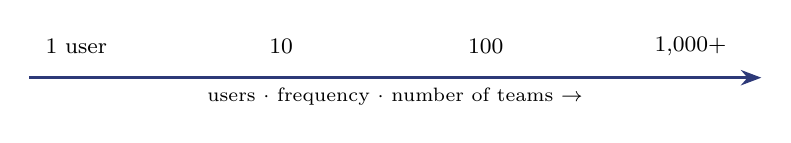
\begin{tikzpicture}
    \foreach \x/\u in {0/{1 user}, 2.6/{10}, 5.2/{100}, 7.8/{1{,}000+}}{
      \node[font=\footnotesize] at (\x,0) {\u};
    }
    \draw[arr] (-0.6,-0.4) -- (8.7,-0.4) node[midway,below,font=\scriptsize]{users $\cdot$ frequency $\cdot$ number of teams $\to$};
  \end{tikzpicture}
  \end{center}
  \begin{block}{Ask three things before you choose}
    \begin{itemize}
      \item \textbf{How many users}, and growing how fast?
      \item \textbf{Who invokes it} --- a human, a schedule, or another service?
      \item \textbf{How many teams} will own and ship pieces of it?
    \end{itemize}
  \end{block}
  {\footnotesize Architecture is not sophistication --- it is matching \emph{structure} to \emph{load}.}
  \note{%
    \textbf{$\sim$8 min.} Point: architecture is a response to \emph{load}, not a measure of skill. Set that frame now or the whole deck reads as a ladder to climb.\\[2pt]
    The three questions are the actual deliverable of this slide --- users, invoker, team count. Notice the third is organisational: architecture tends to mirror team boundaries, which is why a two-person team should almost never build microservices.\\[2pt]
    \textbf{Ask the room:} ``Your churn model runs once a month for one analyst. What architecture?'' A script. Let someone argue for an API and then ask who would call it.\\[2pt]
    \textbf{The failure mode to name early:} engineers choose architecture by what is interesting, not by load.
  }
\end{frame}

% ============================================================
\section{Patterns}
% ============================================================
\begin{frame}{Four patterns of growing complexity}
  \begin{center}
  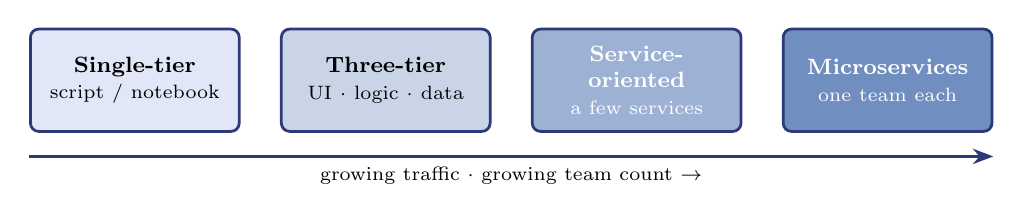
\begin{tikzpicture}
    \node[box, fill=hsbilight,   text width=2.3cm, minimum height=1.3cm] (a) {\textbf{Single-tier}\\ \scriptsize script / notebook};
    \node[box, fill=hsbimid!30,  text width=2.3cm, minimum height=1.3cm, right=0.5cm of a] (b) {\textbf{Three-tier}\\ \scriptsize UI $\cdot$ logic $\cdot$ data};
    \node[box, fill=hsbimid!55,  text width=2.3cm, minimum height=1.3cm, right=0.5cm of b, text=white] (c) {\textbf{Service-oriented}\\ \scriptsize a few services};
    \node[box, fill=hsbimid!80,  text width=2.3cm, minimum height=1.3cm, right=0.5cm of c, text=white] (d) {\textbf{Microservices}\\ \scriptsize one team each};
    \draw[arr] ($(a.south west)+(0,-0.3)$) -- ($(d.south east)+(0,-0.3)$)
      node[midway,below,font=\scriptsize]{growing traffic $\cdot$ growing team count $\to$};
  \end{tikzpicture}
  \end{center}
  {\footnotesize Read left to right as \emph{growing load}, not ``primitive to advanced''. The simplest workable choice wins.}
  \note{%
    \textbf{$\sim$8 min.} Point: four shapes, increasing in operational cost. Read the footnote aloud --- students instinctively read the arrow as a maturity ladder and conclude their notebook is embarrassing.\\[2pt]
    Give the one-line trigger for each: single-tier until someone else needs it; three-tier when a non-developer must use it; services when a \emph{second team} needs to ship independently; microservices when many teams do.\\[2pt]
    \textbf{Every step right costs you} deployment, monitoring, network failure modes and debugging across process boundaries. Nothing is free, and none of it is model work.\\[2pt]
    Most of this course --- and most real analytics work --- lives happily in the first two boxes.
  }
\end{frame}

\begin{frame}{Three-tier --- the workhorse for interactive AI features}
  \begin{center}
  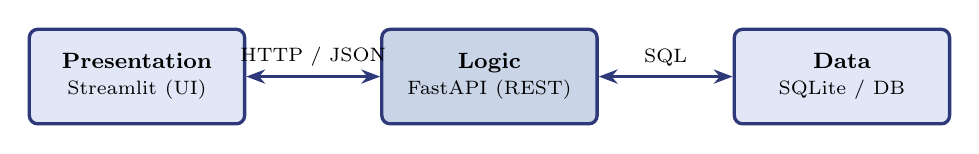
\begin{tikzpicture}
    \node[tier, fill=hsbilight]  (p) {\textbf{Presentation}\\ \scriptsize Streamlit (UI)};
    \node[tier, fill=hsbimid!30, right=1.7cm of p] (l) {\textbf{Logic}\\ \scriptsize FastAPI (REST)};
    \node[tier, fill=hsbilight,  right=1.7cm of l] (d) {\textbf{Data}\\ \scriptsize SQLite / DB};
    \draw[arr,{Stealth[length=2.4mm]}-{Stealth[length=2.4mm]}] (p)--(l) node[midway,above,font=\scriptsize]{HTTP / JSON};
    \draw[arr,{Stealth[length=2.4mm]}-{Stealth[length=2.4mm]}] (l)--(d) node[midway,above,font=\scriptsize]{SQL};
  \end{tikzpicture}
  \end{center}
  \begin{itemize}
    \item Each tier can change independently; the \textbf{REST contract} is the boundary.
    \item The API is reusable --- a second UI, a CLI, or another team can call it.
    \item \emph{You build exactly this} in \textbf{Notebook 34 (POC 2)}.
  \end{itemize}
  \note{%
    \textbf{$\sim$10 min --- the workhorse pattern; spend time here.}\\[2pt]
    Point: three tiers, and the \textbf{REST contract} is the real boundary. Once the contract is fixed, the tiers can be rewritten independently --- that is the entire benefit.\\[2pt]
    The reusability bullet is the one that convinces people: the same API serves the Streamlit UI, a CLI, a scheduled job, and another team, at no extra cost. A notebook serves exactly one consumer.\\[2pt]
    \textbf{Ask the room:} ``Why can't the UI just query the database directly?'' Because then business logic lives in two places and drifts --- and every new consumer re-implements it. That is the whole argument for a logic tier.\\[2pt]
    Promise them NB 34: they build this exact shape, Streamlit $+$ FastAPI $+$ SQLite.
  }
\end{frame}

\begin{frame}{The over-engineering trap}
  \begin{alertblock}{Microservices for a 5-user pilot}
    Microservices became fashionable around 2015; many teams adopted them \emph{before} they had the team size or traffic to justify the operational cost. The right unit of a service is a \emph{capability} --- not every Python module.
  \end{alertblock}
  \begin{exampleblock}{The rule}
    Pick the architecture you'll have \emph{outgrown in 12 months}, not the one you'll \emph{need in 36}. Premature complexity kills more projects than migrations do.
  \end{exampleblock}
  \note{%
    \textbf{$\sim$8 min.} Point: the 12-month rule is the takeaway of the section. Say it twice.\\[2pt]
    The reasoning: you cannot predict 36 months, migrations are far cheaper than people fear, and complexity you don't need yet is paid for every single day in the meantime.\\[2pt]
    \textbf{The unit-of-service line matters:} a service should be a \emph{capability} (``scoring'', ``ingestion''), not a Python module. Teams that split by file end up with a distributed monolith --- all the network cost, none of the independence.\\[2pt]
    \textbf{Ask the room:} ``What's the cost of being wrong in each direction?'' Under-engineering is a bad week when you migrate; over-engineering is a bad year, every year.
  }
\end{frame}

% ============================================================
\section{Frontend \& backend}
% ============================================================
\begin{frame}{Frontend $\leftrightarrow$ backend: the request/response cycle}
  \begin{center}
  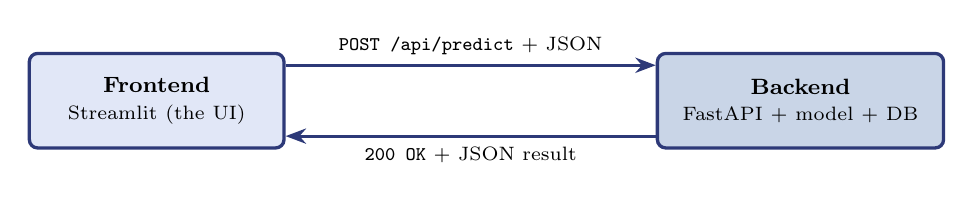
\begin{tikzpicture}
    \node[tier, fill=hsbilight, text width=3.0cm] (fe) {\textbf{Frontend}\\ \scriptsize Streamlit (the UI)};
    \node[tier, fill=hsbimid!30, text width=3.4cm, right=4.7cm of fe] (be) {\textbf{Backend}\\ \scriptsize FastAPI $+$ model $+$ DB};
    \draw[arr] ([yshift=4.5mm]fe.east) -- ([yshift=4.5mm]be.west)
      node[midway,above,font=\scriptsize]{\texttt{POST /api/predict} $+$ JSON};
    \draw[arr] ([yshift=-4.5mm]be.west) -- ([yshift=-4.5mm]fe.east)
      node[midway,below,font=\scriptsize]{\texttt{200 OK} $+$ JSON result};
  \end{tikzpicture}
  \end{center}
  \begin{itemize}
    \item The frontend \emph{never} touches the database --- it only calls the backend over \textbf{HTTP}.
    \item A request names an \textbf{endpoint} (URL path) $+$ a \textbf{verb} (\texttt{GET} read, \texttt{POST} send data) $+$ a JSON \textbf{body}.
    \item The backend validates, runs the logic / model, and returns \textbf{JSON} $+$ a \textbf{status code} (\texttt{200} ok $\cdot$ \texttt{4xx} client error $\cdot$ \texttt{5xx} server error).
  \end{itemize}
  \note{%
    \textbf{$\sim$10 min.} Point: this is the mechanical picture behind ``the tiers talk over HTTP.'' For many students this is the first time client/server is made concrete.\\[2pt]
    Walk one request end to end, out loud: user clicks $\to$ frontend builds JSON $\to$ POST to the endpoint $\to$ backend validates $\to$ model runs $\to$ JSON back with 200 $\to$ UI renders. Then walk a \emph{failure}: bad input $\to$ 422, model crash $\to$ 500.\\[2pt]
    \textbf{The status-code distinction is worth drilling:} 4xx means \emph{you} sent something wrong, 5xx means \emph{I} broke. Students conflate them constantly, and it determines who debugs.\\[2pt]
    First bullet is the security point: the frontend never touches the database. It runs on the user's machine and cannot be trusted with credentials.
  }
\end{frame}

\begin{frame}[fragile]{The backend --- one FastAPI endpoint}
\begin{lstlisting}[style=py]
from fastapi import FastAPI
from pydantic import BaseModel

app = FastAPI()

class Customer(BaseModel):        # validates the incoming JSON
    tenure: int
    monthly_charges: float

@app.post("/api/predict")         # endpoint path + HTTP verb
def predict(c: Customer):
    p = model.predict_proba([[c.tenure, c.monthly_charges]])[0][1]
    return {"churn_probability": round(float(p), 3)}
\end{lstlisting}
  \vspace{-2pt}
  {\footnotesize Pydantic \textbf{validates} the body automatically; returning a dict is serialised to JSON; interactive docs appear free at \texttt{/docs}.}
  \note{%
    \textbf{$\sim$8 min.} Point: a real endpoint is about ten lines. Show that the ceremony they imagine isn't there.\\[2pt]
    Read it in the order the request arrives: the \texttt{Customer} class \emph{is} the contract, the decorator binds path $+$ verb, the body is ordinary Python, the returned dict becomes JSON.\\[2pt]
    \textbf{The Pydantic point is the one worth dwelling on:} you declared types, and got validation free --- send a string where an int belongs and FastAPI returns a 422 with a precise message before your code ever runs. That is the 4xx from the previous slide, generated for you.\\[2pt]
    \textbf{Demo /docs if you're live} --- interactive documentation generated from those type hints is the moment FastAPI sells itself.
  }
\end{frame}

\begin{frame}[fragile]{The frontend --- calling the backend}
\begin{lstlisting}[style=py]
import requests, streamlit as st

resp = requests.post(
    "http://localhost:8000/api/predict",
    json={"tenure": 12, "monthly_charges": 79.9},
    timeout=10,
)
resp.raise_for_status()           # turn 4xx / 5xx into an error
st.metric("Churn risk", resp.json()["churn_probability"])
\end{lstlisting}
  \begin{itemize}
    \item The frontend is just an \textbf{HTTP client} --- the same \texttt{requests} pattern as NB 12.
    \item \textbf{CORS:} a browser blocks cross-origin calls --- add FastAPI's \texttt{CORSMiddleware} so the UI (port 8501) may call the API (port 8000).
  \end{itemize}
  {\footnotesize You build this end-to-end in \textbf{Notebook 34 (POC 2)} --- Streamlit $+$ FastAPI $+$ SQLite.}
  \note{%
    \textbf{$\sim$8 min.} Point: the frontend is \emph{just an HTTP client} --- the same \texttt{requests} they already met in NB 12. Nothing new is being learned; it's being reused.\\[2pt]
    \texttt{raise\_for\_status()} is the line students omit and then spend an hour debugging: without it a 500 sails through and you render an error page's body as data. Insist on it. Same for \texttt{timeout} --- a hung request with no timeout hangs forever.\\[2pt]
    \textbf{CORS will bite them in NB 34}, so plant it now: the browser --- not FastAPI --- blocks the cross-origin call, which is why the error appears in the browser console and the server log looks clean. Knowing where to look saves the hour.\\[2pt]
    \textbf{Ask the room:} ``The UI shows nothing and the server log looks fine. Where do you look first?''
  }
\end{frame}

% ============================================================
\section{Pipeline}
% ============================================================
\begin{frame}{The cross-cutting ML / AI pipeline}
  \begin{center}
  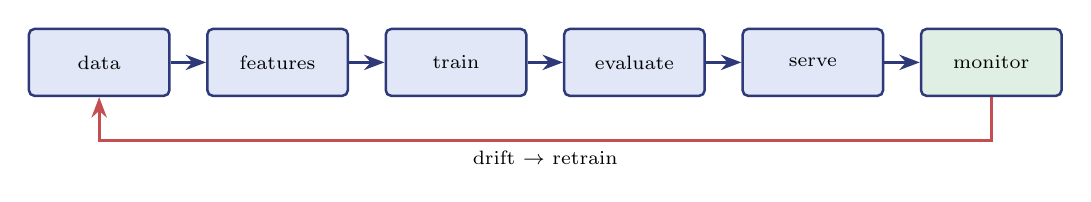
\begin{tikzpicture}
    \node[flow] (d) {data};
    \node[flow, right=0.45cm of d] (f) {features};
    \node[flow, right=0.45cm of f] (t) {train};
    \node[flow, right=0.45cm of t] (e) {evaluate};
    \node[flow, right=0.45cm of e] (s) {serve};
    \node[flow, right=0.45cm of s, fill=cgreen!18] (m) {monitor};
    \foreach \x/\y in {d/f,f/t,t/e,e/s,s/m}{\draw[arr] (\x)--(\y);}
    \draw[arr, draw=cred] (m.south) -- ++(0,-0.55) -| (d.south)
      node[pos=0.25,below,font=\scriptsize]{drift $\to$ retrain};
  \end{tikzpicture}
  \end{center}
  \begin{block}{What pure-software patterns don't capture}
    \begin{itemize}
      \item \textbf{Training data is part of the artefact} --- different snapshot, different product.
      \item \textbf{Drift exists} --- 92\,\% in March is not 92\,\% in October.
      \item \textbf{The feedback loop has economic cost} --- each prediction nudges the next training batch.
    \end{itemize}
  \end{block}
  \note{%
    \textbf{$\sim$10 min --- why ML architecture isn't just software architecture.}\\[2pt]
    Point: the three bullets are what a software-architecture course would miss entirely.\\[2pt]
    \textbf{``Training data is part of the artefact''} is the one to labour: the same code with a different data snapshot is a different product, which is why reproducibility needs data versioning, not just Git.\\[2pt]
    \textbf{The red drift arrow is the slide's spine} --- monitor feeds back to data. Software ships and is done; a model starts decaying on day one because the world moves. 92\,\% in March is not 92\,\% in October.\\[2pt]
    Connect forward: this loop is Module 13 (production) and NB 32 (observability); the question of \emph{which} change moved the metric is Module 18.\\[2pt]
    The feedback bullet is subtle --- if your predictions influence behaviour, they contaminate the next training set. Mention briefly; don't derail.
  }
\end{frame}

% ============================================================
\section{Choosing}
% ============================================================
\begin{frame}{Choosing the right size}
  \begin{block}{Smells that you've outgrown your current shape}
    \begin{itemize}
      \item ``Can we run this nightly?'' $\to$ add scheduling (single-tier job).
      \item A non-developer needs to use it $\to$ add a UI tier (three-tier).
      \item A second team wants to build on it $\to$ expose it as a service.
    \end{itemize}
  \end{block}
  \begin{exampleblock}{Two opposite mistakes}
    \textcolor{cred}{Over-engineering} (microservices for a pilot) and \textcolor{cred}{under-engineering} (a 200-user system held together by one notebook).
  \end{exampleblock}
  \note{%
    \textbf{$\sim$8 min.} Point: don't choose architecture up front --- let \emph{smells} tell you when you've outgrown the current shape.\\[2pt]
    Each smell maps to one move, and the move is small. That's the reassurance: you are never trapped, so choosing simple now is safe.\\[2pt]
    \textbf{Give under-engineering equal air time.} This deck spends more words on over-engineering, but a 200-user system running from one person's notebook is just as real a failure --- and more common in analytics teams. The tell is a single point of failure wearing a lanyard.\\[2pt]
    \textbf{Ask the room:} ``What's the smell that says you've outgrown a notebook?'' Best answer: someone else needs to run it, or it must run when you're on holiday.
  }
\end{frame}

% ============================================================
\section{Course map}
% ============================================================
\begin{frame}{How the course maps to these patterns}
  \small
  \begin{center}
  \begin{tabular}{ll}
    \toprule
    \textbf{Pattern} & \textbf{Where it appears in the course} \\
    \midrule
    Single-tier (script / notebook) & Almost every notebook in the course, by default \\
    Scheduled single-tier           & NB 46 --- scheduling \& orchestration \\
    Three-tier with AI in the middle& NB 34 (POC 2) and the NB 48 capstone \\
    Service-oriented                & \texttt{llm\_providers.py} --- pluggable providers \\
    Microservices                   & \emph{patterns only} --- too big for a teaching course \\
    ML pipeline                     & NB 17--19 $+$ NB 45--46 --- train / evaluate / serve \\
    ML pipeline, deep-learning variant & NB 20--22 --- train / regularise / export (TorchScript) \\
    \bottomrule
  \end{tabular}
  \end{center}
  \vspace{4pt}
  {\footnotesize You \emph{build} the three-tier and ML-pipeline shapes in \textbf{Notebook 34}; the rest you meet as patterns here.}
  \note{%
    \textbf{$\sim$6 min --- close.} Point: they have already been using these patterns without naming them. That's the satisfying reveal.\\[2pt]
    Note honestly that microservices are \emph{patterns only} in this course --- you cannot teach them meaningfully without multiple teams and real traffic, and pretending otherwise would be dishonest.\\[2pt]
    \texttt{llm\_providers.py} is a nice concrete callback: the pluggable-provider shim they've used all course \emph{is} a service-oriented boundary --- one interface, swappable implementations, no caller changes.\\[2pt]
    \textbf{Send them to Notebook 50}, then NB 34 to build it. Next lecture: NB 51, AI-assisted software development.
  }
\end{frame}

\end{document}
"
\ifdefined\notesmode
  \usepackage{pgfpages}
  \setbeameroption{show notes on second screen=right}
\fi

\usetheme{Madrid}
\usecolortheme{default}
\setbeamertemplate{navigation symbols}{}
\setbeamertemplate{footline}[frame number]
\setbeamertemplate{blocks}[rounded][shadow=false]
\setbeamertemplate{headline}{%
  \leavevmode%
  \hbox{%
    \begin{beamercolorbox}[wd=\paperwidth,ht=2.5ex,dp=1.125ex]{section in head/foot}%
      \insertsectionnavigationhorizontal{\paperwidth}{}{\hskip0pt plus1filll}%
    \end{beamercolorbox}%
  }%
}
\AtBeginSection[]{%
  \begin{frame}{Outline}
    \tableofcontents[currentsection,sectionstyle=show/shaded,subsectionstyle=show/show/hide]
  \end{frame}
}

\definecolor{hsbiblue}{RGB}{45,57,120}
\definecolor{hsbimid}{RGB}{76,114,176}
\definecolor{hsbilight}{RGB}{225,231,247}
\definecolor{cgreen}{RGB}{85,164,103}
\definecolor{corange}{RGB}{221,132,82}
\definecolor{cred}{RGB}{196,78,82}
\definecolor{cpurple}{RGB}{129,114,178}
\tikzset{
  box/.style={rounded corners=3pt, draw=hsbiblue, line width=1pt, fill=hsbilight, align=center, inner sep=5pt, font=\footnotesize},
  tier/.style={rounded corners=3pt, draw=hsbiblue, line width=1.2pt, fill=hsbilight, align=center, text width=2.5cm, minimum height=1.2cm, font=\footnotesize},
  flow/.style={rounded corners=2pt, draw=hsbiblue, line width=0.9pt, fill=hsbilight, align=center, text width=1.55cm, minimum height=0.85cm, font=\scriptsize},
  arr/.style={-{Stealth[length=2.6mm]}, line width=1pt, draw=hsbiblue},
}

% ---- Python code listings ----------------------------------
\usepackage{listings}
\lstdefinestyle{py}{%
  language=Python,
  basicstyle=\ttfamily\footnotesize,
  keywordstyle=\color{hsbiblue}\bfseries,
  commentstyle=\color{gray}\itshape,
  stringstyle=\color{cgreen!60!black},
  showstringspaces=false,
  columns=fullflexible,
  breaklines=true,
  aboveskip=3pt, belowskip=1pt,
}

\title{Architecture Patterns for AI Applications}
\subtitle{Module 16 --- Business AI in Practice $\cdot$ Notebook 50}
\author{Prof.\ Dr.\ Christoph Weisser}
\institute{HSBI}
\date{Summer Semester 2026}

\begin{document}

\begin{frame}\titlepage\end{frame}

\begin{frame}{Contents}
  \tableofcontents[hideallsubsections]
\end{frame}

% ============================================================
\section{Traffic}
% ============================================================
\begin{frame}{Architecture is the answer to a \emph{traffic} question}
  \begin{center}
  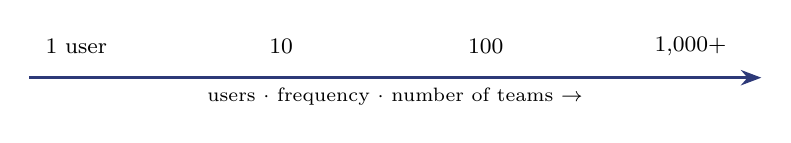
\begin{tikzpicture}
    \foreach \x/\u in {0/{1 user}, 2.6/{10}, 5.2/{100}, 7.8/{1{,}000+}}{
      \node[font=\footnotesize] at (\x,0) {\u};
    }
    \draw[arr] (-0.6,-0.4) -- (8.7,-0.4) node[midway,below,font=\scriptsize]{users $\cdot$ frequency $\cdot$ number of teams $\to$};
  \end{tikzpicture}
  \end{center}
  \begin{block}{Ask three things before you choose}
    \begin{itemize}
      \item \textbf{How many users}, and growing how fast?
      \item \textbf{Who invokes it} --- a human, a schedule, or another service?
      \item \textbf{How many teams} will own and ship pieces of it?
    \end{itemize}
  \end{block}
  {\footnotesize Architecture is not sophistication --- it is matching \emph{structure} to \emph{load}.}
  \note{%
    \textbf{$\sim$8 min.} Point: architecture is a response to \emph{load}, not a measure of skill. Set that frame now or the whole deck reads as a ladder to climb.\\[2pt]
    The three questions are the actual deliverable of this slide --- users, invoker, team count. Notice the third is organisational: architecture tends to mirror team boundaries, which is why a two-person team should almost never build microservices.\\[2pt]
    \textbf{Ask the room:} ``Your churn model runs once a month for one analyst. What architecture?'' A script. Let someone argue for an API and then ask who would call it.\\[2pt]
    \textbf{The failure mode to name early:} engineers choose architecture by what is interesting, not by load.
  }
\end{frame}

% ============================================================
\section{Patterns}
% ============================================================
\begin{frame}{Four patterns of growing complexity}
  \begin{center}
  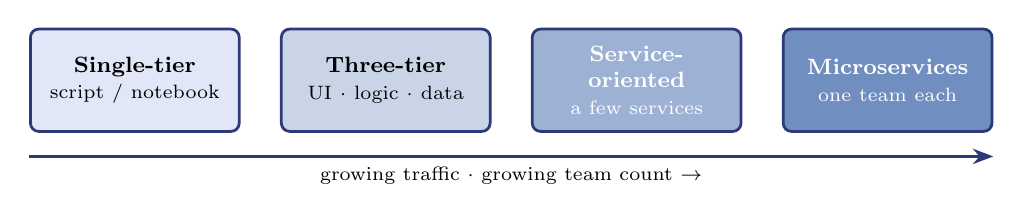
\begin{tikzpicture}
    \node[box, fill=hsbilight,   text width=2.3cm, minimum height=1.3cm] (a) {\textbf{Single-tier}\\ \scriptsize script / notebook};
    \node[box, fill=hsbimid!30,  text width=2.3cm, minimum height=1.3cm, right=0.5cm of a] (b) {\textbf{Three-tier}\\ \scriptsize UI $\cdot$ logic $\cdot$ data};
    \node[box, fill=hsbimid!55,  text width=2.3cm, minimum height=1.3cm, right=0.5cm of b, text=white] (c) {\textbf{Service-oriented}\\ \scriptsize a few services};
    \node[box, fill=hsbimid!80,  text width=2.3cm, minimum height=1.3cm, right=0.5cm of c, text=white] (d) {\textbf{Microservices}\\ \scriptsize one team each};
    \draw[arr] ($(a.south west)+(0,-0.3)$) -- ($(d.south east)+(0,-0.3)$)
      node[midway,below,font=\scriptsize]{growing traffic $\cdot$ growing team count $\to$};
  \end{tikzpicture}
  \end{center}
  {\footnotesize Read left to right as \emph{growing load}, not ``primitive to advanced''. The simplest workable choice wins.}
  \note{%
    \textbf{$\sim$8 min.} Point: four shapes, increasing in operational cost. Read the footnote aloud --- students instinctively read the arrow as a maturity ladder and conclude their notebook is embarrassing.\\[2pt]
    Give the one-line trigger for each: single-tier until someone else needs it; three-tier when a non-developer must use it; services when a \emph{second team} needs to ship independently; microservices when many teams do.\\[2pt]
    \textbf{Every step right costs you} deployment, monitoring, network failure modes and debugging across process boundaries. Nothing is free, and none of it is model work.\\[2pt]
    Most of this course --- and most real analytics work --- lives happily in the first two boxes.
  }
\end{frame}

\begin{frame}{Three-tier --- the workhorse for interactive AI features}
  \begin{center}
  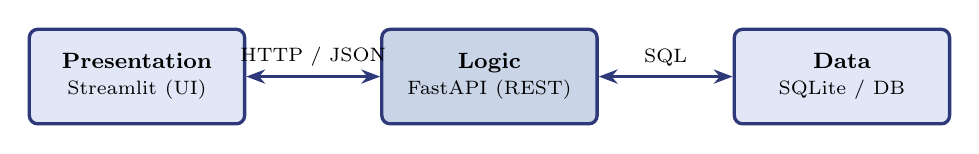
\begin{tikzpicture}
    \node[tier, fill=hsbilight]  (p) {\textbf{Presentation}\\ \scriptsize Streamlit (UI)};
    \node[tier, fill=hsbimid!30, right=1.7cm of p] (l) {\textbf{Logic}\\ \scriptsize FastAPI (REST)};
    \node[tier, fill=hsbilight,  right=1.7cm of l] (d) {\textbf{Data}\\ \scriptsize SQLite / DB};
    \draw[arr,{Stealth[length=2.4mm]}-{Stealth[length=2.4mm]}] (p)--(l) node[midway,above,font=\scriptsize]{HTTP / JSON};
    \draw[arr,{Stealth[length=2.4mm]}-{Stealth[length=2.4mm]}] (l)--(d) node[midway,above,font=\scriptsize]{SQL};
  \end{tikzpicture}
  \end{center}
  \begin{itemize}
    \item Each tier can change independently; the \textbf{REST contract} is the boundary.
    \item The API is reusable --- a second UI, a CLI, or another team can call it.
    \item \emph{You build exactly this} in \textbf{Notebook 34 (POC 2)}.
  \end{itemize}
  \note{%
    \textbf{$\sim$10 min --- the workhorse pattern; spend time here.}\\[2pt]
    Point: three tiers, and the \textbf{REST contract} is the real boundary. Once the contract is fixed, the tiers can be rewritten independently --- that is the entire benefit.\\[2pt]
    The reusability bullet is the one that convinces people: the same API serves the Streamlit UI, a CLI, a scheduled job, and another team, at no extra cost. A notebook serves exactly one consumer.\\[2pt]
    \textbf{Ask the room:} ``Why can't the UI just query the database directly?'' Because then business logic lives in two places and drifts --- and every new consumer re-implements it. That is the whole argument for a logic tier.\\[2pt]
    Promise them NB 34: they build this exact shape, Streamlit $+$ FastAPI $+$ SQLite.
  }
\end{frame}

\begin{frame}{The over-engineering trap}
  \begin{alertblock}{Microservices for a 5-user pilot}
    Microservices became fashionable around 2015; many teams adopted them \emph{before} they had the team size or traffic to justify the operational cost. The right unit of a service is a \emph{capability} --- not every Python module.
  \end{alertblock}
  \begin{exampleblock}{The rule}
    Pick the architecture you'll have \emph{outgrown in 12 months}, not the one you'll \emph{need in 36}. Premature complexity kills more projects than migrations do.
  \end{exampleblock}
  \note{%
    \textbf{$\sim$8 min.} Point: the 12-month rule is the takeaway of the section. Say it twice.\\[2pt]
    The reasoning: you cannot predict 36 months, migrations are far cheaper than people fear, and complexity you don't need yet is paid for every single day in the meantime.\\[2pt]
    \textbf{The unit-of-service line matters:} a service should be a \emph{capability} (``scoring'', ``ingestion''), not a Python module. Teams that split by file end up with a distributed monolith --- all the network cost, none of the independence.\\[2pt]
    \textbf{Ask the room:} ``What's the cost of being wrong in each direction?'' Under-engineering is a bad week when you migrate; over-engineering is a bad year, every year.
  }
\end{frame}

% ============================================================
\section{Frontend \& backend}
% ============================================================
\begin{frame}{Frontend $\leftrightarrow$ backend: the request/response cycle}
  \begin{center}
  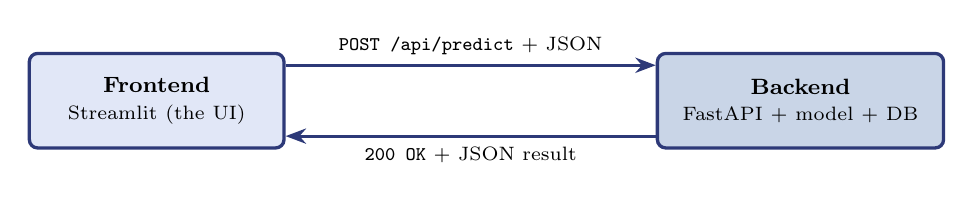
\begin{tikzpicture}
    \node[tier, fill=hsbilight, text width=3.0cm] (fe) {\textbf{Frontend}\\ \scriptsize Streamlit (the UI)};
    \node[tier, fill=hsbimid!30, text width=3.4cm, right=4.7cm of fe] (be) {\textbf{Backend}\\ \scriptsize FastAPI $+$ model $+$ DB};
    \draw[arr] ([yshift=4.5mm]fe.east) -- ([yshift=4.5mm]be.west)
      node[midway,above,font=\scriptsize]{\texttt{POST /api/predict} $+$ JSON};
    \draw[arr] ([yshift=-4.5mm]be.west) -- ([yshift=-4.5mm]fe.east)
      node[midway,below,font=\scriptsize]{\texttt{200 OK} $+$ JSON result};
  \end{tikzpicture}
  \end{center}
  \begin{itemize}
    \item The frontend \emph{never} touches the database --- it only calls the backend over \textbf{HTTP}.
    \item A request names an \textbf{endpoint} (URL path) $+$ a \textbf{verb} (\texttt{GET} read, \texttt{POST} send data) $+$ a JSON \textbf{body}.
    \item The backend validates, runs the logic / model, and returns \textbf{JSON} $+$ a \textbf{status code} (\texttt{200} ok $\cdot$ \texttt{4xx} client error $\cdot$ \texttt{5xx} server error).
  \end{itemize}
  \note{%
    \textbf{$\sim$10 min.} Point: this is the mechanical picture behind ``the tiers talk over HTTP.'' For many students this is the first time client/server is made concrete.\\[2pt]
    Walk one request end to end, out loud: user clicks $\to$ frontend builds JSON $\to$ POST to the endpoint $\to$ backend validates $\to$ model runs $\to$ JSON back with 200 $\to$ UI renders. Then walk a \emph{failure}: bad input $\to$ 422, model crash $\to$ 500.\\[2pt]
    \textbf{The status-code distinction is worth drilling:} 4xx means \emph{you} sent something wrong, 5xx means \emph{I} broke. Students conflate them constantly, and it determines who debugs.\\[2pt]
    First bullet is the security point: the frontend never touches the database. It runs on the user's machine and cannot be trusted with credentials.
  }
\end{frame}

\begin{frame}[fragile]{The backend --- one FastAPI endpoint}
\begin{lstlisting}[style=py]
from fastapi import FastAPI
from pydantic import BaseModel

app = FastAPI()

class Customer(BaseModel):        # validates the incoming JSON
    tenure: int
    monthly_charges: float

@app.post("/api/predict")         # endpoint path + HTTP verb
def predict(c: Customer):
    p = model.predict_proba([[c.tenure, c.monthly_charges]])[0][1]
    return {"churn_probability": round(float(p), 3)}
\end{lstlisting}
  \vspace{-2pt}
  {\footnotesize Pydantic \textbf{validates} the body automatically; returning a dict is serialised to JSON; interactive docs appear free at \texttt{/docs}.}
  \note{%
    \textbf{$\sim$8 min.} Point: a real endpoint is about ten lines. Show that the ceremony they imagine isn't there.\\[2pt]
    Read it in the order the request arrives: the \texttt{Customer} class \emph{is} the contract, the decorator binds path $+$ verb, the body is ordinary Python, the returned dict becomes JSON.\\[2pt]
    \textbf{The Pydantic point is the one worth dwelling on:} you declared types, and got validation free --- send a string where an int belongs and FastAPI returns a 422 with a precise message before your code ever runs. That is the 4xx from the previous slide, generated for you.\\[2pt]
    \textbf{Demo /docs if you're live} --- interactive documentation generated from those type hints is the moment FastAPI sells itself.
  }
\end{frame}

\begin{frame}[fragile]{The frontend --- calling the backend}
\begin{lstlisting}[style=py]
import requests, streamlit as st

resp = requests.post(
    "http://localhost:8000/api/predict",
    json={"tenure": 12, "monthly_charges": 79.9},
    timeout=10,
)
resp.raise_for_status()           # turn 4xx / 5xx into an error
st.metric("Churn risk", resp.json()["churn_probability"])
\end{lstlisting}
  \begin{itemize}
    \item The frontend is just an \textbf{HTTP client} --- the same \texttt{requests} pattern as NB 12.
    \item \textbf{CORS:} a browser blocks cross-origin calls --- add FastAPI's \texttt{CORSMiddleware} so the UI (port 8501) may call the API (port 8000).
  \end{itemize}
  {\footnotesize You build this end-to-end in \textbf{Notebook 34 (POC 2)} --- Streamlit $+$ FastAPI $+$ SQLite.}
  \note{%
    \textbf{$\sim$8 min.} Point: the frontend is \emph{just an HTTP client} --- the same \texttt{requests} they already met in NB 12. Nothing new is being learned; it's being reused.\\[2pt]
    \texttt{raise\_for\_status()} is the line students omit and then spend an hour debugging: without it a 500 sails through and you render an error page's body as data. Insist on it. Same for \texttt{timeout} --- a hung request with no timeout hangs forever.\\[2pt]
    \textbf{CORS will bite them in NB 34}, so plant it now: the browser --- not FastAPI --- blocks the cross-origin call, which is why the error appears in the browser console and the server log looks clean. Knowing where to look saves the hour.\\[2pt]
    \textbf{Ask the room:} ``The UI shows nothing and the server log looks fine. Where do you look first?''
  }
\end{frame}

% ============================================================
\section{Pipeline}
% ============================================================
\begin{frame}{The cross-cutting ML / AI pipeline}
  \begin{center}
  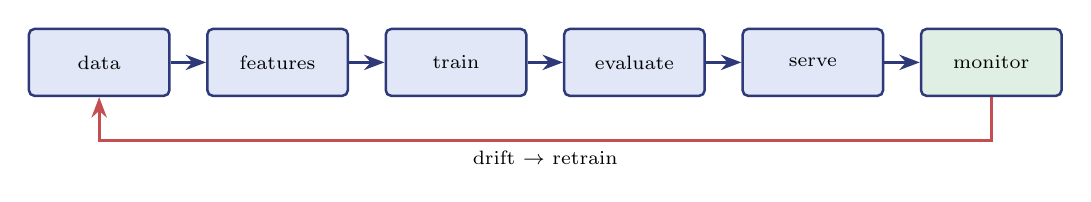
\begin{tikzpicture}
    \node[flow] (d) {data};
    \node[flow, right=0.45cm of d] (f) {features};
    \node[flow, right=0.45cm of f] (t) {train};
    \node[flow, right=0.45cm of t] (e) {evaluate};
    \node[flow, right=0.45cm of e] (s) {serve};
    \node[flow, right=0.45cm of s, fill=cgreen!18] (m) {monitor};
    \foreach \x/\y in {d/f,f/t,t/e,e/s,s/m}{\draw[arr] (\x)--(\y);}
    \draw[arr, draw=cred] (m.south) -- ++(0,-0.55) -| (d.south)
      node[pos=0.25,below,font=\scriptsize]{drift $\to$ retrain};
  \end{tikzpicture}
  \end{center}
  \begin{block}{What pure-software patterns don't capture}
    \begin{itemize}
      \item \textbf{Training data is part of the artefact} --- different snapshot, different product.
      \item \textbf{Drift exists} --- 92\,\% in March is not 92\,\% in October.
      \item \textbf{The feedback loop has economic cost} --- each prediction nudges the next training batch.
    \end{itemize}
  \end{block}
  \note{%
    \textbf{$\sim$10 min --- why ML architecture isn't just software architecture.}\\[2pt]
    Point: the three bullets are what a software-architecture course would miss entirely.\\[2pt]
    \textbf{``Training data is part of the artefact''} is the one to labour: the same code with a different data snapshot is a different product, which is why reproducibility needs data versioning, not just Git.\\[2pt]
    \textbf{The red drift arrow is the slide's spine} --- monitor feeds back to data. Software ships and is done; a model starts decaying on day one because the world moves. 92\,\% in March is not 92\,\% in October.\\[2pt]
    Connect forward: this loop is Module 13 (production) and NB 32 (observability); the question of \emph{which} change moved the metric is Module 18.\\[2pt]
    The feedback bullet is subtle --- if your predictions influence behaviour, they contaminate the next training set. Mention briefly; don't derail.
  }
\end{frame}

% ============================================================
\section{Choosing}
% ============================================================
\begin{frame}{Choosing the right size}
  \begin{block}{Smells that you've outgrown your current shape}
    \begin{itemize}
      \item ``Can we run this nightly?'' $\to$ add scheduling (single-tier job).
      \item A non-developer needs to use it $\to$ add a UI tier (three-tier).
      \item A second team wants to build on it $\to$ expose it as a service.
    \end{itemize}
  \end{block}
  \begin{exampleblock}{Two opposite mistakes}
    \textcolor{cred}{Over-engineering} (microservices for a pilot) and \textcolor{cred}{under-engineering} (a 200-user system held together by one notebook).
  \end{exampleblock}
  \note{%
    \textbf{$\sim$8 min.} Point: don't choose architecture up front --- let \emph{smells} tell you when you've outgrown the current shape.\\[2pt]
    Each smell maps to one move, and the move is small. That's the reassurance: you are never trapped, so choosing simple now is safe.\\[2pt]
    \textbf{Give under-engineering equal air time.} This deck spends more words on over-engineering, but a 200-user system running from one person's notebook is just as real a failure --- and more common in analytics teams. The tell is a single point of failure wearing a lanyard.\\[2pt]
    \textbf{Ask the room:} ``What's the smell that says you've outgrown a notebook?'' Best answer: someone else needs to run it, or it must run when you're on holiday.
  }
\end{frame}

% ============================================================
\section{Course map}
% ============================================================
\begin{frame}{How the course maps to these patterns}
  \small
  \begin{center}
  \begin{tabular}{ll}
    \toprule
    \textbf{Pattern} & \textbf{Where it appears in the course} \\
    \midrule
    Single-tier (script / notebook) & Almost every notebook in the course, by default \\
    Scheduled single-tier           & NB 46 --- scheduling \& orchestration \\
    Three-tier with AI in the middle& NB 34 (POC 2) and the NB 48 capstone \\
    Service-oriented                & \texttt{llm\_providers.py} --- pluggable providers \\
    Microservices                   & \emph{patterns only} --- too big for a teaching course \\
    ML pipeline                     & NB 17--19 $+$ NB 45--46 --- train / evaluate / serve \\
    ML pipeline, deep-learning variant & NB 20--22 --- train / regularise / export (TorchScript) \\
    \bottomrule
  \end{tabular}
  \end{center}
  \vspace{4pt}
  {\footnotesize You \emph{build} the three-tier and ML-pipeline shapes in \textbf{Notebook 34}; the rest you meet as patterns here.}
  \note{%
    \textbf{$\sim$6 min --- close.} Point: they have already been using these patterns without naming them. That's the satisfying reveal.\\[2pt]
    Note honestly that microservices are \emph{patterns only} in this course --- you cannot teach them meaningfully without multiple teams and real traffic, and pretending otherwise would be dishonest.\\[2pt]
    \texttt{llm\_providers.py} is a nice concrete callback: the pluggable-provider shim they've used all course \emph{is} a service-oriented boundary --- one interface, swappable implementations, no caller changes.\\[2pt]
    \textbf{Send them to Notebook 50}, then NB 34 to build it. Next lecture: NB 51, AI-assisted software development.
  }
\end{frame}

\end{document}
"
\ifdefined\notesmode
  \usepackage{pgfpages}
  \setbeameroption{show notes on second screen=right}
\fi

\usetheme{Madrid}
\usecolortheme{default}
\setbeamertemplate{navigation symbols}{}
\setbeamertemplate{footline}[frame number]
\setbeamertemplate{blocks}[rounded][shadow=false]
\setbeamertemplate{headline}{%
  \leavevmode%
  \hbox{%
    \begin{beamercolorbox}[wd=\paperwidth,ht=2.5ex,dp=1.125ex]{section in head/foot}%
      \insertsectionnavigationhorizontal{\paperwidth}{}{\hskip0pt plus1filll}%
    \end{beamercolorbox}%
  }%
}
\AtBeginSection[]{%
  \begin{frame}{Outline}
    \tableofcontents[currentsection,sectionstyle=show/shaded,subsectionstyle=show/show/hide]
  \end{frame}
}

\definecolor{hsbiblue}{RGB}{45,57,120}
\definecolor{hsbimid}{RGB}{76,114,176}
\definecolor{hsbilight}{RGB}{225,231,247}
\definecolor{cgreen}{RGB}{85,164,103}
\definecolor{corange}{RGB}{221,132,82}
\definecolor{cred}{RGB}{196,78,82}
\definecolor{cpurple}{RGB}{129,114,178}
\tikzset{
  box/.style={rounded corners=3pt, draw=hsbiblue, line width=1pt, fill=hsbilight, align=center, inner sep=5pt, font=\footnotesize},
  tier/.style={rounded corners=3pt, draw=hsbiblue, line width=1.2pt, fill=hsbilight, align=center, text width=2.5cm, minimum height=1.2cm, font=\footnotesize},
  flow/.style={rounded corners=2pt, draw=hsbiblue, line width=0.9pt, fill=hsbilight, align=center, text width=1.55cm, minimum height=0.85cm, font=\scriptsize},
  arr/.style={-{Stealth[length=2.6mm]}, line width=1pt, draw=hsbiblue},
}

% ---- Python code listings ----------------------------------
\usepackage{listings}
\lstdefinestyle{py}{%
  language=Python,
  basicstyle=\ttfamily\footnotesize,
  keywordstyle=\color{hsbiblue}\bfseries,
  commentstyle=\color{gray}\itshape,
  stringstyle=\color{cgreen!60!black},
  showstringspaces=false,
  columns=fullflexible,
  breaklines=true,
  aboveskip=3pt, belowskip=1pt,
}

\title{Architecture Patterns for AI Applications}
\subtitle{Module 16 --- Business AI in Practice $\cdot$ Notebook 50}
\author{Prof.\ Dr.\ Christoph Weisser}
\institute{HSBI}
\date{Summer Semester 2026}

\begin{document}

\begin{frame}\titlepage\end{frame}

\begin{frame}{Contents}
  \tableofcontents[hideallsubsections]
\end{frame}

% ============================================================
\section{Traffic}
% ============================================================
\begin{frame}{Architecture is the answer to a \emph{traffic} question}
  \begin{center}
  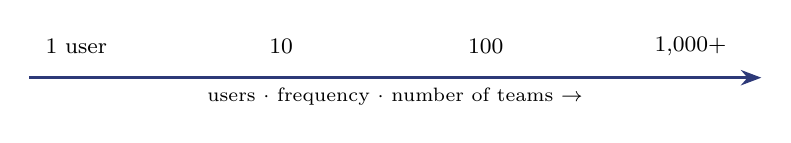
\begin{tikzpicture}
    \foreach \x/\u in {0/{1 user}, 2.6/{10}, 5.2/{100}, 7.8/{1{,}000+}}{
      \node[font=\footnotesize] at (\x,0) {\u};
    }
    \draw[arr] (-0.6,-0.4) -- (8.7,-0.4) node[midway,below,font=\scriptsize]{users $\cdot$ frequency $\cdot$ number of teams $\to$};
  \end{tikzpicture}
  \end{center}
  \begin{block}{Ask three things before you choose}
    \begin{itemize}
      \item \textbf{How many users}, and growing how fast?
      \item \textbf{Who invokes it} --- a human, a schedule, or another service?
      \item \textbf{How many teams} will own and ship pieces of it?
    \end{itemize}
  \end{block}
  {\footnotesize Architecture is not sophistication --- it is matching \emph{structure} to \emph{load}.}
  \note{%
    \textbf{$\sim$8 min.} Point: architecture is a response to \emph{load}, not a measure of skill. Set that frame now or the whole deck reads as a ladder to climb.\\[2pt]
    The three questions are the actual deliverable of this slide --- users, invoker, team count. Notice the third is organisational: architecture tends to mirror team boundaries, which is why a two-person team should almost never build microservices.\\[2pt]
    \textbf{Ask the room:} ``Your churn model runs once a month for one analyst. What architecture?'' A script. Let someone argue for an API and then ask who would call it.\\[2pt]
    \textbf{The failure mode to name early:} engineers choose architecture by what is interesting, not by load.
  }
\end{frame}

% ============================================================
\section{Patterns}
% ============================================================
\begin{frame}{Four patterns of growing complexity}
  \begin{center}
  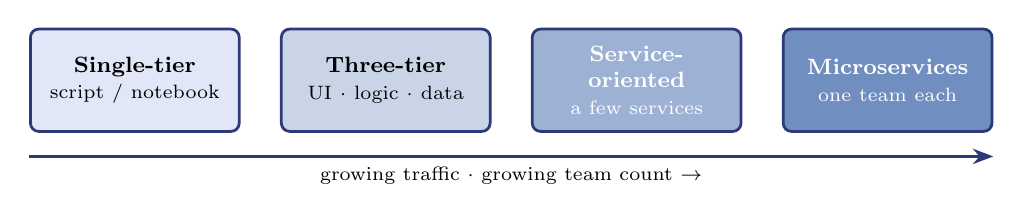
\begin{tikzpicture}
    \node[box, fill=hsbilight,   text width=2.3cm, minimum height=1.3cm] (a) {\textbf{Single-tier}\\ \scriptsize script / notebook};
    \node[box, fill=hsbimid!30,  text width=2.3cm, minimum height=1.3cm, right=0.5cm of a] (b) {\textbf{Three-tier}\\ \scriptsize UI $\cdot$ logic $\cdot$ data};
    \node[box, fill=hsbimid!55,  text width=2.3cm, minimum height=1.3cm, right=0.5cm of b, text=white] (c) {\textbf{Service-oriented}\\ \scriptsize a few services};
    \node[box, fill=hsbimid!80,  text width=2.3cm, minimum height=1.3cm, right=0.5cm of c, text=white] (d) {\textbf{Microservices}\\ \scriptsize one team each};
    \draw[arr] ($(a.south west)+(0,-0.3)$) -- ($(d.south east)+(0,-0.3)$)
      node[midway,below,font=\scriptsize]{growing traffic $\cdot$ growing team count $\to$};
  \end{tikzpicture}
  \end{center}
  {\footnotesize Read left to right as \emph{growing load}, not ``primitive to advanced''. The simplest workable choice wins.}
  \note{%
    \textbf{$\sim$8 min.} Point: four shapes, increasing in operational cost. Read the footnote aloud --- students instinctively read the arrow as a maturity ladder and conclude their notebook is embarrassing.\\[2pt]
    Give the one-line trigger for each: single-tier until someone else needs it; three-tier when a non-developer must use it; services when a \emph{second team} needs to ship independently; microservices when many teams do.\\[2pt]
    \textbf{Every step right costs you} deployment, monitoring, network failure modes and debugging across process boundaries. Nothing is free, and none of it is model work.\\[2pt]
    Most of this course --- and most real analytics work --- lives happily in the first two boxes.
  }
\end{frame}

\begin{frame}{Three-tier --- the workhorse for interactive AI features}
  \begin{center}
  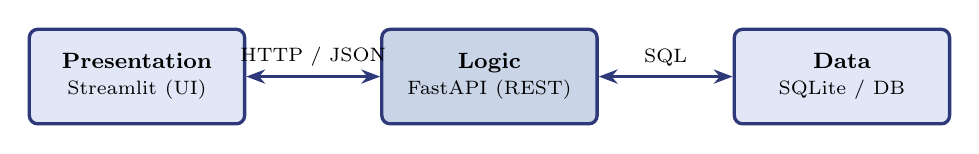
\begin{tikzpicture}
    \node[tier, fill=hsbilight]  (p) {\textbf{Presentation}\\ \scriptsize Streamlit (UI)};
    \node[tier, fill=hsbimid!30, right=1.7cm of p] (l) {\textbf{Logic}\\ \scriptsize FastAPI (REST)};
    \node[tier, fill=hsbilight,  right=1.7cm of l] (d) {\textbf{Data}\\ \scriptsize SQLite / DB};
    \draw[arr,{Stealth[length=2.4mm]}-{Stealth[length=2.4mm]}] (p)--(l) node[midway,above,font=\scriptsize]{HTTP / JSON};
    \draw[arr,{Stealth[length=2.4mm]}-{Stealth[length=2.4mm]}] (l)--(d) node[midway,above,font=\scriptsize]{SQL};
  \end{tikzpicture}
  \end{center}
  \begin{itemize}
    \item Each tier can change independently; the \textbf{REST contract} is the boundary.
    \item The API is reusable --- a second UI, a CLI, or another team can call it.
    \item \emph{You build exactly this} in \textbf{Notebook 34 (POC 2)}.
  \end{itemize}
  \note{%
    \textbf{$\sim$10 min --- the workhorse pattern; spend time here.}\\[2pt]
    Point: three tiers, and the \textbf{REST contract} is the real boundary. Once the contract is fixed, the tiers can be rewritten independently --- that is the entire benefit.\\[2pt]
    The reusability bullet is the one that convinces people: the same API serves the Streamlit UI, a CLI, a scheduled job, and another team, at no extra cost. A notebook serves exactly one consumer.\\[2pt]
    \textbf{Ask the room:} ``Why can't the UI just query the database directly?'' Because then business logic lives in two places and drifts --- and every new consumer re-implements it. That is the whole argument for a logic tier.\\[2pt]
    Promise them NB 34: they build this exact shape, Streamlit $+$ FastAPI $+$ SQLite.
  }
\end{frame}

\begin{frame}{The over-engineering trap}
  \begin{alertblock}{Microservices for a 5-user pilot}
    Microservices became fashionable around 2015; many teams adopted them \emph{before} they had the team size or traffic to justify the operational cost. The right unit of a service is a \emph{capability} --- not every Python module.
  \end{alertblock}
  \begin{exampleblock}{The rule}
    Pick the architecture you'll have \emph{outgrown in 12 months}, not the one you'll \emph{need in 36}. Premature complexity kills more projects than migrations do.
  \end{exampleblock}
  \note{%
    \textbf{$\sim$8 min.} Point: the 12-month rule is the takeaway of the section. Say it twice.\\[2pt]
    The reasoning: you cannot predict 36 months, migrations are far cheaper than people fear, and complexity you don't need yet is paid for every single day in the meantime.\\[2pt]
    \textbf{The unit-of-service line matters:} a service should be a \emph{capability} (``scoring'', ``ingestion''), not a Python module. Teams that split by file end up with a distributed monolith --- all the network cost, none of the independence.\\[2pt]
    \textbf{Ask the room:} ``What's the cost of being wrong in each direction?'' Under-engineering is a bad week when you migrate; over-engineering is a bad year, every year.
  }
\end{frame}

% ============================================================
\section{Frontend \& backend}
% ============================================================
\begin{frame}{Frontend $\leftrightarrow$ backend: the request/response cycle}
  \begin{center}
  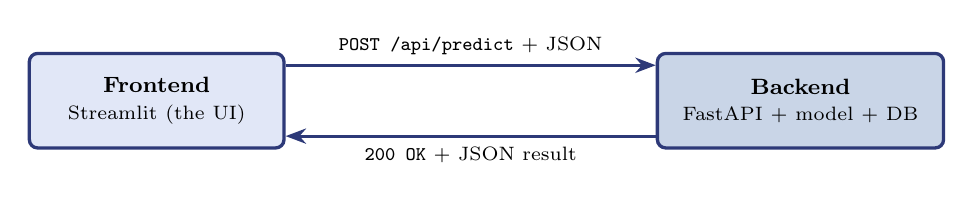
\begin{tikzpicture}
    \node[tier, fill=hsbilight, text width=3.0cm] (fe) {\textbf{Frontend}\\ \scriptsize Streamlit (the UI)};
    \node[tier, fill=hsbimid!30, text width=3.4cm, right=4.7cm of fe] (be) {\textbf{Backend}\\ \scriptsize FastAPI $+$ model $+$ DB};
    \draw[arr] ([yshift=4.5mm]fe.east) -- ([yshift=4.5mm]be.west)
      node[midway,above,font=\scriptsize]{\texttt{POST /api/predict} $+$ JSON};
    \draw[arr] ([yshift=-4.5mm]be.west) -- ([yshift=-4.5mm]fe.east)
      node[midway,below,font=\scriptsize]{\texttt{200 OK} $+$ JSON result};
  \end{tikzpicture}
  \end{center}
  \begin{itemize}
    \item The frontend \emph{never} touches the database --- it only calls the backend over \textbf{HTTP}.
    \item A request names an \textbf{endpoint} (URL path) $+$ a \textbf{verb} (\texttt{GET} read, \texttt{POST} send data) $+$ a JSON \textbf{body}.
    \item The backend validates, runs the logic / model, and returns \textbf{JSON} $+$ a \textbf{status code} (\texttt{200} ok $\cdot$ \texttt{4xx} client error $\cdot$ \texttt{5xx} server error).
  \end{itemize}
  \note{%
    \textbf{$\sim$10 min.} Point: this is the mechanical picture behind ``the tiers talk over HTTP.'' For many students this is the first time client/server is made concrete.\\[2pt]
    Walk one request end to end, out loud: user clicks $\to$ frontend builds JSON $\to$ POST to the endpoint $\to$ backend validates $\to$ model runs $\to$ JSON back with 200 $\to$ UI renders. Then walk a \emph{failure}: bad input $\to$ 422, model crash $\to$ 500.\\[2pt]
    \textbf{The status-code distinction is worth drilling:} 4xx means \emph{you} sent something wrong, 5xx means \emph{I} broke. Students conflate them constantly, and it determines who debugs.\\[2pt]
    First bullet is the security point: the frontend never touches the database. It runs on the user's machine and cannot be trusted with credentials.
  }
\end{frame}

\begin{frame}[fragile]{The backend --- one FastAPI endpoint}
\begin{lstlisting}[style=py]
from fastapi import FastAPI
from pydantic import BaseModel

app = FastAPI()

class Customer(BaseModel):        # validates the incoming JSON
    tenure: int
    monthly_charges: float

@app.post("/api/predict")         # endpoint path + HTTP verb
def predict(c: Customer):
    p = model.predict_proba([[c.tenure, c.monthly_charges]])[0][1]
    return {"churn_probability": round(float(p), 3)}
\end{lstlisting}
  \vspace{-2pt}
  {\footnotesize Pydantic \textbf{validates} the body automatically; returning a dict is serialised to JSON; interactive docs appear free at \texttt{/docs}.}
  \note{%
    \textbf{$\sim$8 min.} Point: a real endpoint is about ten lines. Show that the ceremony they imagine isn't there.\\[2pt]
    Read it in the order the request arrives: the \texttt{Customer} class \emph{is} the contract, the decorator binds path $+$ verb, the body is ordinary Python, the returned dict becomes JSON.\\[2pt]
    \textbf{The Pydantic point is the one worth dwelling on:} you declared types, and got validation free --- send a string where an int belongs and FastAPI returns a 422 with a precise message before your code ever runs. That is the 4xx from the previous slide, generated for you.\\[2pt]
    \textbf{Demo /docs if you're live} --- interactive documentation generated from those type hints is the moment FastAPI sells itself.
  }
\end{frame}

\begin{frame}[fragile]{The frontend --- calling the backend}
\begin{lstlisting}[style=py]
import requests, streamlit as st

resp = requests.post(
    "http://localhost:8000/api/predict",
    json={"tenure": 12, "monthly_charges": 79.9},
    timeout=10,
)
resp.raise_for_status()           # turn 4xx / 5xx into an error
st.metric("Churn risk", resp.json()["churn_probability"])
\end{lstlisting}
  \begin{itemize}
    \item The frontend is just an \textbf{HTTP client} --- the same \texttt{requests} pattern as NB 12.
    \item \textbf{CORS:} a browser blocks cross-origin calls --- add FastAPI's \texttt{CORSMiddleware} so the UI (port 8501) may call the API (port 8000).
  \end{itemize}
  {\footnotesize You build this end-to-end in \textbf{Notebook 34 (POC 2)} --- Streamlit $+$ FastAPI $+$ SQLite.}
  \note{%
    \textbf{$\sim$8 min.} Point: the frontend is \emph{just an HTTP client} --- the same \texttt{requests} they already met in NB 12. Nothing new is being learned; it's being reused.\\[2pt]
    \texttt{raise\_for\_status()} is the line students omit and then spend an hour debugging: without it a 500 sails through and you render an error page's body as data. Insist on it. Same for \texttt{timeout} --- a hung request with no timeout hangs forever.\\[2pt]
    \textbf{CORS will bite them in NB 34}, so plant it now: the browser --- not FastAPI --- blocks the cross-origin call, which is why the error appears in the browser console and the server log looks clean. Knowing where to look saves the hour.\\[2pt]
    \textbf{Ask the room:} ``The UI shows nothing and the server log looks fine. Where do you look first?''
  }
\end{frame}

% ============================================================
\section{Pipeline}
% ============================================================
\begin{frame}{The cross-cutting ML / AI pipeline}
  \begin{center}
  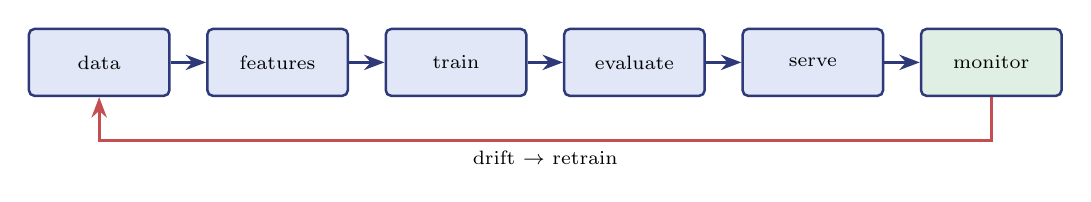
\begin{tikzpicture}
    \node[flow] (d) {data};
    \node[flow, right=0.45cm of d] (f) {features};
    \node[flow, right=0.45cm of f] (t) {train};
    \node[flow, right=0.45cm of t] (e) {evaluate};
    \node[flow, right=0.45cm of e] (s) {serve};
    \node[flow, right=0.45cm of s, fill=cgreen!18] (m) {monitor};
    \foreach \x/\y in {d/f,f/t,t/e,e/s,s/m}{\draw[arr] (\x)--(\y);}
    \draw[arr, draw=cred] (m.south) -- ++(0,-0.55) -| (d.south)
      node[pos=0.25,below,font=\scriptsize]{drift $\to$ retrain};
  \end{tikzpicture}
  \end{center}
  \begin{block}{What pure-software patterns don't capture}
    \begin{itemize}
      \item \textbf{Training data is part of the artefact} --- different snapshot, different product.
      \item \textbf{Drift exists} --- 92\,\% in March is not 92\,\% in October.
      \item \textbf{The feedback loop has economic cost} --- each prediction nudges the next training batch.
    \end{itemize}
  \end{block}
  \note{%
    \textbf{$\sim$10 min --- why ML architecture isn't just software architecture.}\\[2pt]
    Point: the three bullets are what a software-architecture course would miss entirely.\\[2pt]
    \textbf{``Training data is part of the artefact''} is the one to labour: the same code with a different data snapshot is a different product, which is why reproducibility needs data versioning, not just Git.\\[2pt]
    \textbf{The red drift arrow is the slide's spine} --- monitor feeds back to data. Software ships and is done; a model starts decaying on day one because the world moves. 92\,\% in March is not 92\,\% in October.\\[2pt]
    Connect forward: this loop is Module 13 (production) and NB 32 (observability); the question of \emph{which} change moved the metric is Module 18.\\[2pt]
    The feedback bullet is subtle --- if your predictions influence behaviour, they contaminate the next training set. Mention briefly; don't derail.
  }
\end{frame}

% ============================================================
\section{Choosing}
% ============================================================
\begin{frame}{Choosing the right size}
  \begin{block}{Smells that you've outgrown your current shape}
    \begin{itemize}
      \item ``Can we run this nightly?'' $\to$ add scheduling (single-tier job).
      \item A non-developer needs to use it $\to$ add a UI tier (three-tier).
      \item A second team wants to build on it $\to$ expose it as a service.
    \end{itemize}
  \end{block}
  \begin{exampleblock}{Two opposite mistakes}
    \textcolor{cred}{Over-engineering} (microservices for a pilot) and \textcolor{cred}{under-engineering} (a 200-user system held together by one notebook).
  \end{exampleblock}
  \note{%
    \textbf{$\sim$8 min.} Point: don't choose architecture up front --- let \emph{smells} tell you when you've outgrown the current shape.\\[2pt]
    Each smell maps to one move, and the move is small. That's the reassurance: you are never trapped, so choosing simple now is safe.\\[2pt]
    \textbf{Give under-engineering equal air time.} This deck spends more words on over-engineering, but a 200-user system running from one person's notebook is just as real a failure --- and more common in analytics teams. The tell is a single point of failure wearing a lanyard.\\[2pt]
    \textbf{Ask the room:} ``What's the smell that says you've outgrown a notebook?'' Best answer: someone else needs to run it, or it must run when you're on holiday.
  }
\end{frame}

% ============================================================
\section{Course map}
% ============================================================
\begin{frame}{How the course maps to these patterns}
  \small
  \begin{center}
  \begin{tabular}{ll}
    \toprule
    \textbf{Pattern} & \textbf{Where it appears in the course} \\
    \midrule
    Single-tier (script / notebook) & Almost every notebook in the course, by default \\
    Scheduled single-tier           & NB 46 --- scheduling \& orchestration \\
    Three-tier with AI in the middle& NB 34 (POC 2) and the NB 48 capstone \\
    Service-oriented                & \texttt{llm\_providers.py} --- pluggable providers \\
    Microservices                   & \emph{patterns only} --- too big for a teaching course \\
    ML pipeline                     & NB 17--19 $+$ NB 45--46 --- train / evaluate / serve \\
    ML pipeline, deep-learning variant & NB 20--22 --- train / regularise / export (TorchScript) \\
    \bottomrule
  \end{tabular}
  \end{center}
  \vspace{4pt}
  {\footnotesize You \emph{build} the three-tier and ML-pipeline shapes in \textbf{Notebook 34}; the rest you meet as patterns here.}
  \note{%
    \textbf{$\sim$6 min --- close.} Point: they have already been using these patterns without naming them. That's the satisfying reveal.\\[2pt]
    Note honestly that microservices are \emph{patterns only} in this course --- you cannot teach them meaningfully without multiple teams and real traffic, and pretending otherwise would be dishonest.\\[2pt]
    \texttt{llm\_providers.py} is a nice concrete callback: the pluggable-provider shim they've used all course \emph{is} a service-oriented boundary --- one interface, swappable implementations, no caller changes.\\[2pt]
    \textbf{Send them to Notebook 50}, then NB 34 to build it. Next lecture: NB 51, AI-assisted software development.
  }
\end{frame}

\end{document}
"
\ifdefined\notesmode
  \usepackage{pgfpages}
  \setbeameroption{show notes on second screen=right}
\fi

\usetheme{Madrid}
\usecolortheme{default}
\setbeamertemplate{navigation symbols}{}
\setbeamertemplate{footline}[frame number]
\setbeamertemplate{blocks}[rounded][shadow=false]
\setbeamertemplate{headline}{%
  \leavevmode%
  \hbox{%
    \begin{beamercolorbox}[wd=\paperwidth,ht=2.5ex,dp=1.125ex]{section in head/foot}%
      \insertsectionnavigationhorizontal{\paperwidth}{}{\hskip0pt plus1filll}%
    \end{beamercolorbox}%
  }%
}
\AtBeginSection[]{%
  \begin{frame}{Outline}
    \tableofcontents[currentsection,sectionstyle=show/shaded,subsectionstyle=show/show/hide]
  \end{frame}
}

\definecolor{hsbiblue}{RGB}{45,57,120}
\definecolor{hsbimid}{RGB}{76,114,176}
\definecolor{hsbilight}{RGB}{225,231,247}
\definecolor{cgreen}{RGB}{85,164,103}
\definecolor{corange}{RGB}{221,132,82}
\definecolor{cred}{RGB}{196,78,82}
\definecolor{cpurple}{RGB}{129,114,178}
\tikzset{
  box/.style={rounded corners=3pt, draw=hsbiblue, line width=1pt, fill=hsbilight, align=center, inner sep=5pt, font=\footnotesize},
  tier/.style={rounded corners=3pt, draw=hsbiblue, line width=1.2pt, fill=hsbilight, align=center, text width=2.5cm, minimum height=1.2cm, font=\footnotesize},
  flow/.style={rounded corners=2pt, draw=hsbiblue, line width=0.9pt, fill=hsbilight, align=center, text width=1.55cm, minimum height=0.85cm, font=\scriptsize},
  arr/.style={-{Stealth[length=2.6mm]}, line width=1pt, draw=hsbiblue},
}

% ---- Python code listings ----------------------------------
\usepackage{listings}
\lstdefinestyle{py}{%
  language=Python,
  basicstyle=\ttfamily\footnotesize,
  keywordstyle=\color{hsbiblue}\bfseries,
  commentstyle=\color{gray}\itshape,
  stringstyle=\color{cgreen!60!black},
  showstringspaces=false,
  columns=fullflexible,
  breaklines=true,
  aboveskip=3pt, belowskip=1pt,
}

\title{Architecture Patterns for AI Applications}
\subtitle{Module 16 --- Business AI in Practice $\cdot$ Notebook 50}
\author{Prof.\ Dr.\ Christoph Weisser}
\institute{HSBI}
\date{Summer Semester 2026}

\begin{document}

\begin{frame}\titlepage\end{frame}

\begin{frame}{Contents}
  \tableofcontents[hideallsubsections]
\end{frame}

% ============================================================
\section{Traffic}
% ============================================================
\begin{frame}{Architecture is the answer to a \emph{traffic} question}
  \begin{center}
  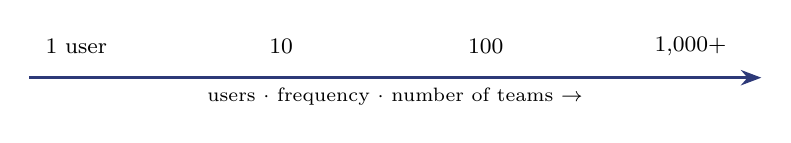
\begin{tikzpicture}
    \foreach \x/\u in {0/{1 user}, 2.6/{10}, 5.2/{100}, 7.8/{1{,}000+}}{
      \node[font=\footnotesize] at (\x,0) {\u};
    }
    \draw[arr] (-0.6,-0.4) -- (8.7,-0.4) node[midway,below,font=\scriptsize]{users $\cdot$ frequency $\cdot$ number of teams $\to$};
  \end{tikzpicture}
  \end{center}
  \begin{block}{Ask three things before you choose}
    \begin{itemize}
      \item \textbf{How many users}, and growing how fast?
      \item \textbf{Who invokes it} --- a human, a schedule, or another service?
      \item \textbf{How many teams} will own and ship pieces of it?
    \end{itemize}
  \end{block}
  {\footnotesize Architecture is not sophistication --- it is matching \emph{structure} to \emph{load}.}
  \note{%
    \textbf{$\sim$8 min.} Point: architecture is a response to \emph{load}, not a measure of skill. Set that frame now or the whole deck reads as a ladder to climb.\\[2pt]
    The three questions are the actual deliverable of this slide --- users, invoker, team count. Notice the third is organisational: architecture tends to mirror team boundaries, which is why a two-person team should almost never build microservices.\\[2pt]
    \textbf{Ask the room:} ``Your churn model runs once a month for one analyst. What architecture?'' A script. Let someone argue for an API and then ask who would call it.\\[2pt]
    \textbf{The failure mode to name early:} engineers choose architecture by what is interesting, not by load.
  }
\end{frame}

% ============================================================
\section{Patterns}
% ============================================================
\begin{frame}{Four patterns of growing complexity}
  \begin{center}
  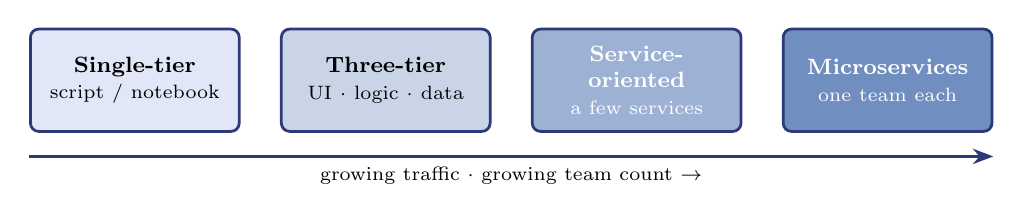
\begin{tikzpicture}
    \node[box, fill=hsbilight,   text width=2.3cm, minimum height=1.3cm] (a) {\textbf{Single-tier}\\ \scriptsize script / notebook};
    \node[box, fill=hsbimid!30,  text width=2.3cm, minimum height=1.3cm, right=0.5cm of a] (b) {\textbf{Three-tier}\\ \scriptsize UI $\cdot$ logic $\cdot$ data};
    \node[box, fill=hsbimid!55,  text width=2.3cm, minimum height=1.3cm, right=0.5cm of b, text=white] (c) {\textbf{Service-oriented}\\ \scriptsize a few services};
    \node[box, fill=hsbimid!80,  text width=2.3cm, minimum height=1.3cm, right=0.5cm of c, text=white] (d) {\textbf{Microservices}\\ \scriptsize one team each};
    \draw[arr] ($(a.south west)+(0,-0.3)$) -- ($(d.south east)+(0,-0.3)$)
      node[midway,below,font=\scriptsize]{growing traffic $\cdot$ growing team count $\to$};
  \end{tikzpicture}
  \end{center}
  {\footnotesize Read left to right as \emph{growing load}, not ``primitive to advanced''. The simplest workable choice wins.}
  \note{%
    \textbf{$\sim$8 min.} Point: four shapes, increasing in operational cost. Read the footnote aloud --- students instinctively read the arrow as a maturity ladder and conclude their notebook is embarrassing.\\[2pt]
    Give the one-line trigger for each: single-tier until someone else needs it; three-tier when a non-developer must use it; services when a \emph{second team} needs to ship independently; microservices when many teams do.\\[2pt]
    \textbf{Every step right costs you} deployment, monitoring, network failure modes and debugging across process boundaries. Nothing is free, and none of it is model work.\\[2pt]
    Most of this course --- and most real analytics work --- lives happily in the first two boxes.
  }
\end{frame}

\begin{frame}{Three-tier --- the workhorse for interactive AI features}
  \begin{center}
  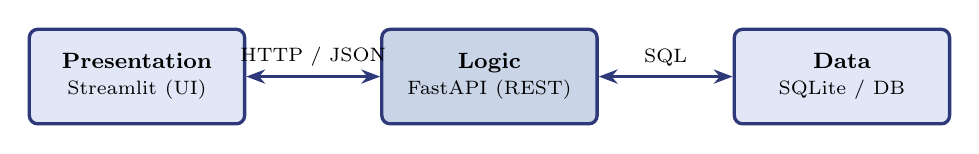
\begin{tikzpicture}
    \node[tier, fill=hsbilight]  (p) {\textbf{Presentation}\\ \scriptsize Streamlit (UI)};
    \node[tier, fill=hsbimid!30, right=1.7cm of p] (l) {\textbf{Logic}\\ \scriptsize FastAPI (REST)};
    \node[tier, fill=hsbilight,  right=1.7cm of l] (d) {\textbf{Data}\\ \scriptsize SQLite / DB};
    \draw[arr,{Stealth[length=2.4mm]}-{Stealth[length=2.4mm]}] (p)--(l) node[midway,above,font=\scriptsize]{HTTP / JSON};
    \draw[arr,{Stealth[length=2.4mm]}-{Stealth[length=2.4mm]}] (l)--(d) node[midway,above,font=\scriptsize]{SQL};
  \end{tikzpicture}
  \end{center}
  \begin{itemize}
    \item Each tier can change independently; the \textbf{REST contract} is the boundary.
    \item The API is reusable --- a second UI, a CLI, or another team can call it.
    \item \emph{You build exactly this} in \textbf{Notebook 34 (POC 2)}.
  \end{itemize}
  \note{%
    \textbf{$\sim$10 min --- the workhorse pattern; spend time here.}\\[2pt]
    Point: three tiers, and the \textbf{REST contract} is the real boundary. Once the contract is fixed, the tiers can be rewritten independently --- that is the entire benefit.\\[2pt]
    The reusability bullet is the one that convinces people: the same API serves the Streamlit UI, a CLI, a scheduled job, and another team, at no extra cost. A notebook serves exactly one consumer.\\[2pt]
    \textbf{Ask the room:} ``Why can't the UI just query the database directly?'' Because then business logic lives in two places and drifts --- and every new consumer re-implements it. That is the whole argument for a logic tier.\\[2pt]
    Promise them NB 34: they build this exact shape, Streamlit $+$ FastAPI $+$ SQLite.
  }
\end{frame}

\begin{frame}{The over-engineering trap}
  \begin{alertblock}{Microservices for a 5-user pilot}
    Microservices became fashionable around 2015; many teams adopted them \emph{before} they had the team size or traffic to justify the operational cost. The right unit of a service is a \emph{capability} --- not every Python module.
  \end{alertblock}
  \begin{exampleblock}{The rule}
    Pick the architecture you'll have \emph{outgrown in 12 months}, not the one you'll \emph{need in 36}. Premature complexity kills more projects than migrations do.
  \end{exampleblock}
  \note{%
    \textbf{$\sim$8 min.} Point: the 12-month rule is the takeaway of the section. Say it twice.\\[2pt]
    The reasoning: you cannot predict 36 months, migrations are far cheaper than people fear, and complexity you don't need yet is paid for every single day in the meantime.\\[2pt]
    \textbf{The unit-of-service line matters:} a service should be a \emph{capability} (``scoring'', ``ingestion''), not a Python module. Teams that split by file end up with a distributed monolith --- all the network cost, none of the independence.\\[2pt]
    \textbf{Ask the room:} ``What's the cost of being wrong in each direction?'' Under-engineering is a bad week when you migrate; over-engineering is a bad year, every year.
  }
\end{frame}

% ============================================================
\section{Frontend \& backend}
% ============================================================
\begin{frame}{Frontend $\leftrightarrow$ backend: the request/response cycle}
  \begin{center}
  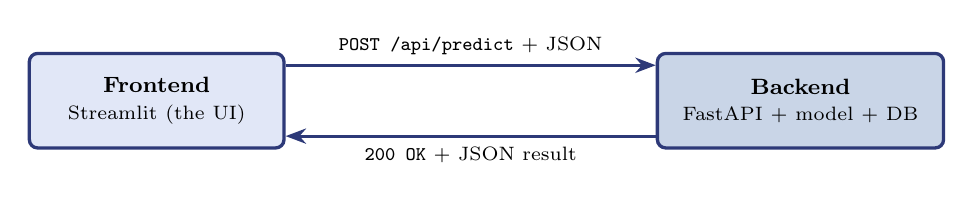
\begin{tikzpicture}
    \node[tier, fill=hsbilight, text width=3.0cm] (fe) {\textbf{Frontend}\\ \scriptsize Streamlit (the UI)};
    \node[tier, fill=hsbimid!30, text width=3.4cm, right=4.7cm of fe] (be) {\textbf{Backend}\\ \scriptsize FastAPI $+$ model $+$ DB};
    \draw[arr] ([yshift=4.5mm]fe.east) -- ([yshift=4.5mm]be.west)
      node[midway,above,font=\scriptsize]{\texttt{POST /api/predict} $+$ JSON};
    \draw[arr] ([yshift=-4.5mm]be.west) -- ([yshift=-4.5mm]fe.east)
      node[midway,below,font=\scriptsize]{\texttt{200 OK} $+$ JSON result};
  \end{tikzpicture}
  \end{center}
  \begin{itemize}
    \item The frontend \emph{never} touches the database --- it only calls the backend over \textbf{HTTP}.
    \item A request names an \textbf{endpoint} (URL path) $+$ a \textbf{verb} (\texttt{GET} read, \texttt{POST} send data) $+$ a JSON \textbf{body}.
    \item The backend validates, runs the logic / model, and returns \textbf{JSON} $+$ a \textbf{status code} (\texttt{200} ok $\cdot$ \texttt{4xx} client error $\cdot$ \texttt{5xx} server error).
  \end{itemize}
  \note{%
    \textbf{$\sim$10 min.} Point: this is the mechanical picture behind ``the tiers talk over HTTP.'' For many students this is the first time client/server is made concrete.\\[2pt]
    Walk one request end to end, out loud: user clicks $\to$ frontend builds JSON $\to$ POST to the endpoint $\to$ backend validates $\to$ model runs $\to$ JSON back with 200 $\to$ UI renders. Then walk a \emph{failure}: bad input $\to$ 422, model crash $\to$ 500.\\[2pt]
    \textbf{The status-code distinction is worth drilling:} 4xx means \emph{you} sent something wrong, 5xx means \emph{I} broke. Students conflate them constantly, and it determines who debugs.\\[2pt]
    First bullet is the security point: the frontend never touches the database. It runs on the user's machine and cannot be trusted with credentials.
  }
\end{frame}

\begin{frame}[fragile]{The backend --- one FastAPI endpoint}
\begin{lstlisting}[style=py]
from fastapi import FastAPI
from pydantic import BaseModel

app = FastAPI()

class Customer(BaseModel):        # validates the incoming JSON
    tenure: int
    monthly_charges: float

@app.post("/api/predict")         # endpoint path + HTTP verb
def predict(c: Customer):
    p = model.predict_proba([[c.tenure, c.monthly_charges]])[0][1]
    return {"churn_probability": round(float(p), 3)}
\end{lstlisting}
  \vspace{-2pt}
  {\footnotesize Pydantic \textbf{validates} the body automatically; returning a dict is serialised to JSON; interactive docs appear free at \texttt{/docs}.}
  \note{%
    \textbf{$\sim$8 min.} Point: a real endpoint is about ten lines. Show that the ceremony they imagine isn't there.\\[2pt]
    Read it in the order the request arrives: the \texttt{Customer} class \emph{is} the contract, the decorator binds path $+$ verb, the body is ordinary Python, the returned dict becomes JSON.\\[2pt]
    \textbf{The Pydantic point is the one worth dwelling on:} you declared types, and got validation free --- send a string where an int belongs and FastAPI returns a 422 with a precise message before your code ever runs. That is the 4xx from the previous slide, generated for you.\\[2pt]
    \textbf{Demo /docs if you're live} --- interactive documentation generated from those type hints is the moment FastAPI sells itself.
  }
\end{frame}

\begin{frame}[fragile]{The frontend --- calling the backend}
\begin{lstlisting}[style=py]
import requests, streamlit as st

resp = requests.post(
    "http://localhost:8000/api/predict",
    json={"tenure": 12, "monthly_charges": 79.9},
    timeout=10,
)
resp.raise_for_status()           # turn 4xx / 5xx into an error
st.metric("Churn risk", resp.json()["churn_probability"])
\end{lstlisting}
  \begin{itemize}
    \item The frontend is just an \textbf{HTTP client} --- the same \texttt{requests} pattern as NB 12.
    \item \textbf{CORS:} a browser blocks cross-origin calls --- add FastAPI's \texttt{CORSMiddleware} so the UI (port 8501) may call the API (port 8000).
  \end{itemize}
  {\footnotesize You build this end-to-end in \textbf{Notebook 34 (POC 2)} --- Streamlit $+$ FastAPI $+$ SQLite.}
  \note{%
    \textbf{$\sim$8 min.} Point: the frontend is \emph{just an HTTP client} --- the same \texttt{requests} they already met in NB 12. Nothing new is being learned; it's being reused.\\[2pt]
    \texttt{raise\_for\_status()} is the line students omit and then spend an hour debugging: without it a 500 sails through and you render an error page's body as data. Insist on it. Same for \texttt{timeout} --- a hung request with no timeout hangs forever.\\[2pt]
    \textbf{CORS will bite them in NB 34}, so plant it now: the browser --- not FastAPI --- blocks the cross-origin call, which is why the error appears in the browser console and the server log looks clean. Knowing where to look saves the hour.\\[2pt]
    \textbf{Ask the room:} ``The UI shows nothing and the server log looks fine. Where do you look first?''
  }
\end{frame}

% ============================================================
\section{Pipeline}
% ============================================================
\begin{frame}{The cross-cutting ML / AI pipeline}
  \begin{center}
  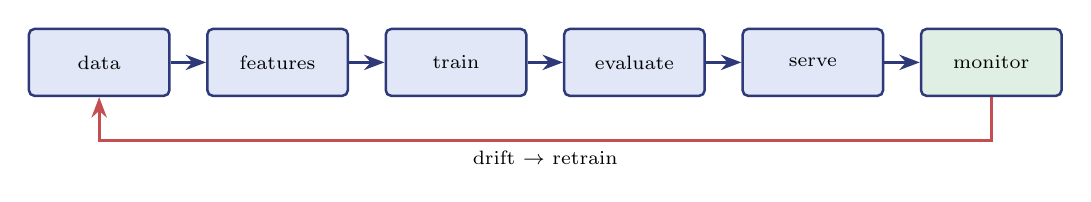
\begin{tikzpicture}
    \node[flow] (d) {data};
    \node[flow, right=0.45cm of d] (f) {features};
    \node[flow, right=0.45cm of f] (t) {train};
    \node[flow, right=0.45cm of t] (e) {evaluate};
    \node[flow, right=0.45cm of e] (s) {serve};
    \node[flow, right=0.45cm of s, fill=cgreen!18] (m) {monitor};
    \foreach \x/\y in {d/f,f/t,t/e,e/s,s/m}{\draw[arr] (\x)--(\y);}
    \draw[arr, draw=cred] (m.south) -- ++(0,-0.55) -| (d.south)
      node[pos=0.25,below,font=\scriptsize]{drift $\to$ retrain};
  \end{tikzpicture}
  \end{center}
  \begin{block}{What pure-software patterns don't capture}
    \begin{itemize}
      \item \textbf{Training data is part of the artefact} --- different snapshot, different product.
      \item \textbf{Drift exists} --- 92\,\% in March is not 92\,\% in October.
      \item \textbf{The feedback loop has economic cost} --- each prediction nudges the next training batch.
    \end{itemize}
  \end{block}
  \note{%
    \textbf{$\sim$10 min --- why ML architecture isn't just software architecture.}\\[2pt]
    Point: the three bullets are what a software-architecture course would miss entirely.\\[2pt]
    \textbf{``Training data is part of the artefact''} is the one to labour: the same code with a different data snapshot is a different product, which is why reproducibility needs data versioning, not just Git.\\[2pt]
    \textbf{The red drift arrow is the slide's spine} --- monitor feeds back to data. Software ships and is done; a model starts decaying on day one because the world moves. 92\,\% in March is not 92\,\% in October.\\[2pt]
    Connect forward: this loop is Module 13 (production) and NB 32 (observability); the question of \emph{which} change moved the metric is Module 18.\\[2pt]
    The feedback bullet is subtle --- if your predictions influence behaviour, they contaminate the next training set. Mention briefly; don't derail.
  }
\end{frame}

% ============================================================
\section{Choosing}
% ============================================================
\begin{frame}{Choosing the right size}
  \begin{block}{Smells that you've outgrown your current shape}
    \begin{itemize}
      \item ``Can we run this nightly?'' $\to$ add scheduling (single-tier job).
      \item A non-developer needs to use it $\to$ add a UI tier (three-tier).
      \item A second team wants to build on it $\to$ expose it as a service.
    \end{itemize}
  \end{block}
  \begin{exampleblock}{Two opposite mistakes}
    \textcolor{cred}{Over-engineering} (microservices for a pilot) and \textcolor{cred}{under-engineering} (a 200-user system held together by one notebook).
  \end{exampleblock}
  \note{%
    \textbf{$\sim$8 min.} Point: don't choose architecture up front --- let \emph{smells} tell you when you've outgrown the current shape.\\[2pt]
    Each smell maps to one move, and the move is small. That's the reassurance: you are never trapped, so choosing simple now is safe.\\[2pt]
    \textbf{Give under-engineering equal air time.} This deck spends more words on over-engineering, but a 200-user system running from one person's notebook is just as real a failure --- and more common in analytics teams. The tell is a single point of failure wearing a lanyard.\\[2pt]
    \textbf{Ask the room:} ``What's the smell that says you've outgrown a notebook?'' Best answer: someone else needs to run it, or it must run when you're on holiday.
  }
\end{frame}

% ============================================================
\section{Course map}
% ============================================================
\begin{frame}{How the course maps to these patterns}
  \small
  \begin{center}
  \begin{tabular}{ll}
    \toprule
    \textbf{Pattern} & \textbf{Where it appears in the course} \\
    \midrule
    Single-tier (script / notebook) & Almost every notebook in the course, by default \\
    Scheduled single-tier           & NB 46 --- scheduling \& orchestration \\
    Three-tier with AI in the middle& NB 34 (POC 2) and the NB 48 capstone \\
    Service-oriented                & \texttt{llm\_providers.py} --- pluggable providers \\
    Microservices                   & \emph{patterns only} --- too big for a teaching course \\
    ML pipeline                     & NB 17--19 $+$ NB 45--46 --- train / evaluate / serve \\
    ML pipeline, deep-learning variant & NB 20--22 --- train / regularise / export (TorchScript) \\
    \bottomrule
  \end{tabular}
  \end{center}
  \vspace{4pt}
  {\footnotesize You \emph{build} the three-tier and ML-pipeline shapes in \textbf{Notebook 34}; the rest you meet as patterns here.}
  \note{%
    \textbf{$\sim$6 min --- close.} Point: they have already been using these patterns without naming them. That's the satisfying reveal.\\[2pt]
    Note honestly that microservices are \emph{patterns only} in this course --- you cannot teach them meaningfully without multiple teams and real traffic, and pretending otherwise would be dishonest.\\[2pt]
    \texttt{llm\_providers.py} is a nice concrete callback: the pluggable-provider shim they've used all course \emph{is} a service-oriented boundary --- one interface, swappable implementations, no caller changes.\\[2pt]
    \textbf{Send them to Notebook 50}, then NB 34 to build it. Next lecture: NB 51, AI-assisted software development.
  }
\end{frame}

\end{document}
